\begin{figure}[H]
    \centering
    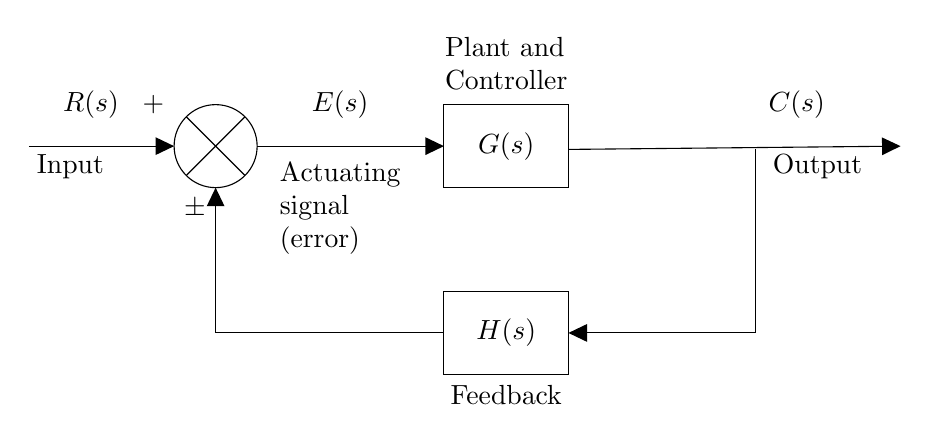
\begin{tikzpicture}[x=0.75pt,y=0.75pt,yscale=-1,xscale=1]
%uncomment if require: \path (0,300); %set diagram left start at 0, and has height of 300

%Straight Lines
\draw    (10,68.71) -- (78,68.71) ;
\draw [shift={(80,68.71)}, rotate = 180] [fill={rgb, 255:red, 0; green, 0; blue, 0 }  ][line width=0.75]  [draw opacity=0] (8.93,-4.29) -- (0,0) -- (8.93,4.29) -- cycle    ;

%Flowchart: Summing Junction
\draw   (80,68.71) .. controls (80,57.67) and (88.95,48.71) .. (100,48.71) .. controls (111.05,48.71) and (120,57.67) .. (120,68.71) .. controls (120,79.76) and (111.05,88.71) .. (100,88.71) .. controls (88.95,88.71) and (80,79.76) .. (80,68.71) -- cycle ; \draw   (85.86,54.57) -- (114.14,82.86) ; \draw   (114.14,54.57) -- (85.86,82.86) ;
%Straight Lines
\draw    (120,68.71) -- (208,68.71) ;
\draw [shift={(210,68.71)}, rotate = 180] [fill={rgb, 255:red, 0; green, 0; blue, 0 }  ][line width=0.75]  [draw opacity=0] (8.93,-4.29) -- (0,0) -- (8.93,4.29) -- cycle    ;

%Shape: Rectangle
\draw   (210,48.71) -- (270,48.71) -- (270,88.71) -- (210,88.71) -- cycle ;
%Straight Lines
\draw    (270,70.29) -- (428,68.73) ;
\draw [shift={(430,68.71)}, rotate = 539.44] [fill={rgb, 255:red, 0; green, 0; blue, 0 }  ][line width=0.75]  [draw opacity=0] (8.93,-4.29) -- (0,0) -- (8.93,4.29) -- cycle    ;

%Straight Lines
\draw    (360,70.29) -- (360,158.71) ;


%Straight Lines
\draw    (360,158.71) -- (272,158.71) ;
\draw [shift={(270,158.71)}, rotate = 360] [fill={rgb, 255:red, 0; green, 0; blue, 0 }  ][line width=0.75]  [draw opacity=0] (8.93,-4.29) -- (0,0) -- (8.93,4.29) -- cycle    ;

%Shape: Rectangle
\draw   (210,138.71) -- (270,138.71) -- (270,178.71) -- (210,178.71) -- cycle ;
%Straight Lines
\draw    (210,158.71) -- (100,158.71) ;


%Straight Lines
\draw    (100,158.71) -- (100,90.71) ;
\draw [shift={(100,88.71)}, rotate = 450] [fill={rgb, 255:red, 0; green, 0; blue, 0 }  ][line width=0.75]  [draw opacity=0] (8.93,-4.29) -- (0,0) -- (8.93,4.29) -- cycle    ;


% Text Node
\draw (40,48.71) node   {$R( s)$};
% Text Node
\draw (70,48.71) node   {$+$};
% Text Node
\draw (160,48.71) node   {$E( s)$};
% Text Node
\draw (240,68.71) node   {$G( s)$};
% Text Node
\draw (380,48.71) node   {$C( s)$};
% Text Node
\draw (240,158.71) node   {$H( s)$};
% Text Node
\draw (90,98.71) node   {$\pm $};
% Text Node
\draw (160,98.71) node  [align=left] {Actuating \\signal\\(error)};
% Text Node
\draw (30,78.71) node  [align=left] {Input};
% Text Node
\draw (390,78.71) node  [align=left] {Output};
% Text Node
\draw (240,188.71) node  [align=left] {Feedback};
% Text Node
\draw (240,28.71) node  [align=left] {Plant and \\Controller};


\end{tikzpicture}
    \caption{Standard format feedback loop here Arrows signify signals and boxes mechanisms, this standard form feedback loop are used to illustrate the golden formula}
    \label{fig:FeedbackLoop}
\end{figure}